\documentclass[a2paper,landscape,fontscale=0.35]{baposter}

\usepackage{preamble}

\begin{document}

\begin{poster}{
	% poster
	columns=3,
	background=user,
	% box header
	headershade=plain,
	headerColorOne=white,
	headerfont=\Large\bfseries,
	headerFontColor=black,
	headerborder=closed,
	% box
	boxshade=plain,
	boxColorOne=white,
	boxopacity=.70,
	textborder=rectangle,
	borderColor=black,
	linewidth=0.5pt,
}
{}
{Compositional Decompilation}
{Robin Eklind}
{
\includegraphics[height=0.05\textheight]{inc/logo.pdf}}

\headerbox{Problem}{column=0, row=0, span=1}
{
	Recover high-level control flow primitives (e.g. if-statements, for-loop, …) from low-level LLVM IR (platform-independent assembly).
}

\headerbox{Method}{column=0, below=auto, span=1}
{
	Identify control flow primitives using subgraph isomorphism search algorithms \cite{decomp_llvm}.

	\begin{figure}[H]
		\centering
		\begin{subfigure}[ht]{0.30\textwidth}
			\lstinputlisting[language=go, style=go, breaklines=false, numbers=none]{inc/if.c}
			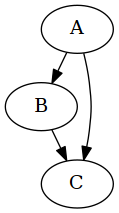
\includegraphics[width=\textwidth]{inc/if.png}
		\end{subfigure}
		\enskip
		\begin{subfigure}[ht]{0.50\textwidth}
			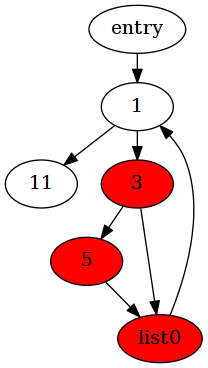
\includegraphics[width=\textwidth]{inc/foo.png}
		\end{subfigure}
		\caption{Pseudo-code and graph representation of an if-statement (left) and the control flow graph of \texttt{main} (right).}
	\end{figure}
}

\headerbox{Results}{name=rbox, column=1, row=0, span=2}
{
	\begin{figure}[H]
		\centering
		\begin{subfigure}[ht]{0.58\textwidth}
			\lstinputlisting[language=llvm, style=nasm, breaklines=false, numbers=none]{inc/foo.ll}
		\end{subfigure}
		\enskip
		\begin{subfigure}[ht]{0.38\textwidth}
			\lstinputlisting[language=go, style=go, tabsize=2, breaklines=false, numbers=none]{inc/foo.go}
		\end{subfigure}
		\caption{LLVM IR input (left) and Go output (right).}
	\end{figure}
}

\headerbox{Source Code}{column=1, below=rbox, span=1}
{
	\url{https://github.com/mewrev/graphs}
	\url{https://github.com/mewrev/ll2dot}
	\url{https://github.com/mewrev/ll2go}
}

\headerbox{References}{column=2, below=rbox, span=1}
{
	\renewcommand{\section}[2]{}
	\bibliography{references}
}

\end{poster}

\end{document}
